\section{Experiments}
\subsection{Datasets and Metrics}
\textbf{CUHK-PEDES}\cite{CUHK-PEDES} serves as a foundational benchmark for research in the text-to-image person retrieval. It comprises 40,206 pedestrian images corresponding to 13,003 distinct identities, with each image accompanied by two independently annotated textual descriptions. Following the official data split, the training set includes 34,054 images and 68,108 textual descriptions covering 11,003 identities. The testing set involves 3,074 images and 6,156 descriptions from 1,000 identities, while a separate validation set consists of 3,078 images from another 1,000 identities.

\noindent\textbf{ICFG-PEDES}\cite{ding2021semantically} is a large-scale text-to-image person retrieval dataset, consisting of  54,522 pedestrian images associated with 4,102 distinct identities. Each image is annotated with a single fine-grained textual description, making it more focused and discriminative than CUHK-PEDES. The dataset is split into a training set with 34,674 image-text pairs from 3,102 identities and a testing set with 19,848 pairs corresponding to the remaining 1,000 identities.

\noindent\textbf{RSTPReid}\cite{zhu2021dssl} is a text-to-image person retrieval dataset designed to reflect real-world surveillance scenarios. It comprises 20,505 pedestrian images collected from 15 distinct cameras, covering 4,101 unique identities. Each identity is represented by five images captured from different viewpoints, and every image is annotated with two textual descriptions, resulting in a total of 41,010 image-text pairs. Following the official dataset protocol, the training set includes 18,505 images and 37,010 descriptions from 3,701 identities. Both the validation and testing sets are composed of 1,000 images and 2,000 descriptions, each corresponding to 200 identities.

\begin{table}[tp]
\caption{Ablation study of our proposed query and gallery feature compensation on the RSTPReid dataset with IRRA baseline.}
\vspace{-0.8em}
\label{tab: ablation}
\centering
\resizebox{0.975\linewidth}{!}{
\begin{tabular}{cc|cc|cccc}
\hline
\multicolumn{2}{c|}{Query} & \multicolumn{2}{c|}{Gallery}  & \multicolumn{4}{c}{RSTPReid} \\ 
$P_{key}$& $P_{diverse}$ & $P_{key}$ &  $P_{diverse}$ & R1 & R5 & R10 & mAP \\
\hline
\ding{55} & \ding{55}& \ding{55} & \ding{55} & 60.20 & 81.30 & 88.20 & 47.17 \\
\ding{52} & \ding{55} & \ding{52} & \ding{55} & 61.80 & 82.95 & 89.30 & 48.40 \\
\ding{55} & \ding{52} & \ding{55} & \ding{52} & 61.90 & 82.00 & 89.50 & 48.58 \\
\ding{55} &\ding{55} & \ding{52} & \ding{52} & 60.95 & 82.95 & 89.25 & 47.95 \\
\ding{52}& \ding{52}& \ding{55} & \ding{55} & 61.35 & 81.75 & 89.15 & 48.43 \\
\rowcolor[HTML]{EAFAF1} 
 \ding{52} &\ding{52}  & \ding{52} & \ding{52} & 63.10 & 82.40 & 89.40 & 49.20 \\
 \hline
\end{tabular}
}
\end{table}

\textbf{Evaluate Metrics.} In line with prior studies \cite{RDE, IRRA}, we employ Rank-k accuracy (with k = 1, 5, 10) and mean Average Precision (mAP) as the primary evaluation metrics across all three datasets. These metrics collectively assess the retrieval accuracy and overall matching quality. A higher value in either Rank-k or mAP indicates superior performance.

\subsection{Implementation Details}
All experiments were conducted on one NVIDIA RTX 4090 GPU and one Intel I9-13900K CPU. For LLM collaborative reformulation, we employed TVI-LFM \cite{hu2024empowering} to generate the caption of the image gallery and Qwen2.5-VL-32B \cite{Qwen2.5-VL} to reformulate query and gallery captions, with the decoding temperature set to 0.01. Specifically, we designed two distinct prompt templates to guide the reformulation process for both queries and image-derived captions. Each template yields 15 reformulated variants (just in one QA), resulting in a total of 30 semantic reformulations per input instance (it can also use less reformulations as show in \ref{fig:tem_scale} (b) for faster speed) 
For empirical comparisons, we adopted four representative baseline methods: IRRA~\cite{IRRA}, RDE~\cite{RDE}, HAM(IRRA)~\cite{HAM}, and HAM(RDE), evaluating each using the default configurations and pretrained weights provided in their official open-source implementations.
The threshold $\delta$ with default -0.03, and it helps retain some neutral words, avoiding overly strict filtering. It is the average of GPT labeled key words of all datasets. The hyperparameter $\alpha$ in Eq.~\ref{eq:alpha} is set to 0.75, and $\beta$ in Eq.~\ref{eq:beta} is set to 0.3, both selected via grid search on the validation set.


\begin{figure}
\centering
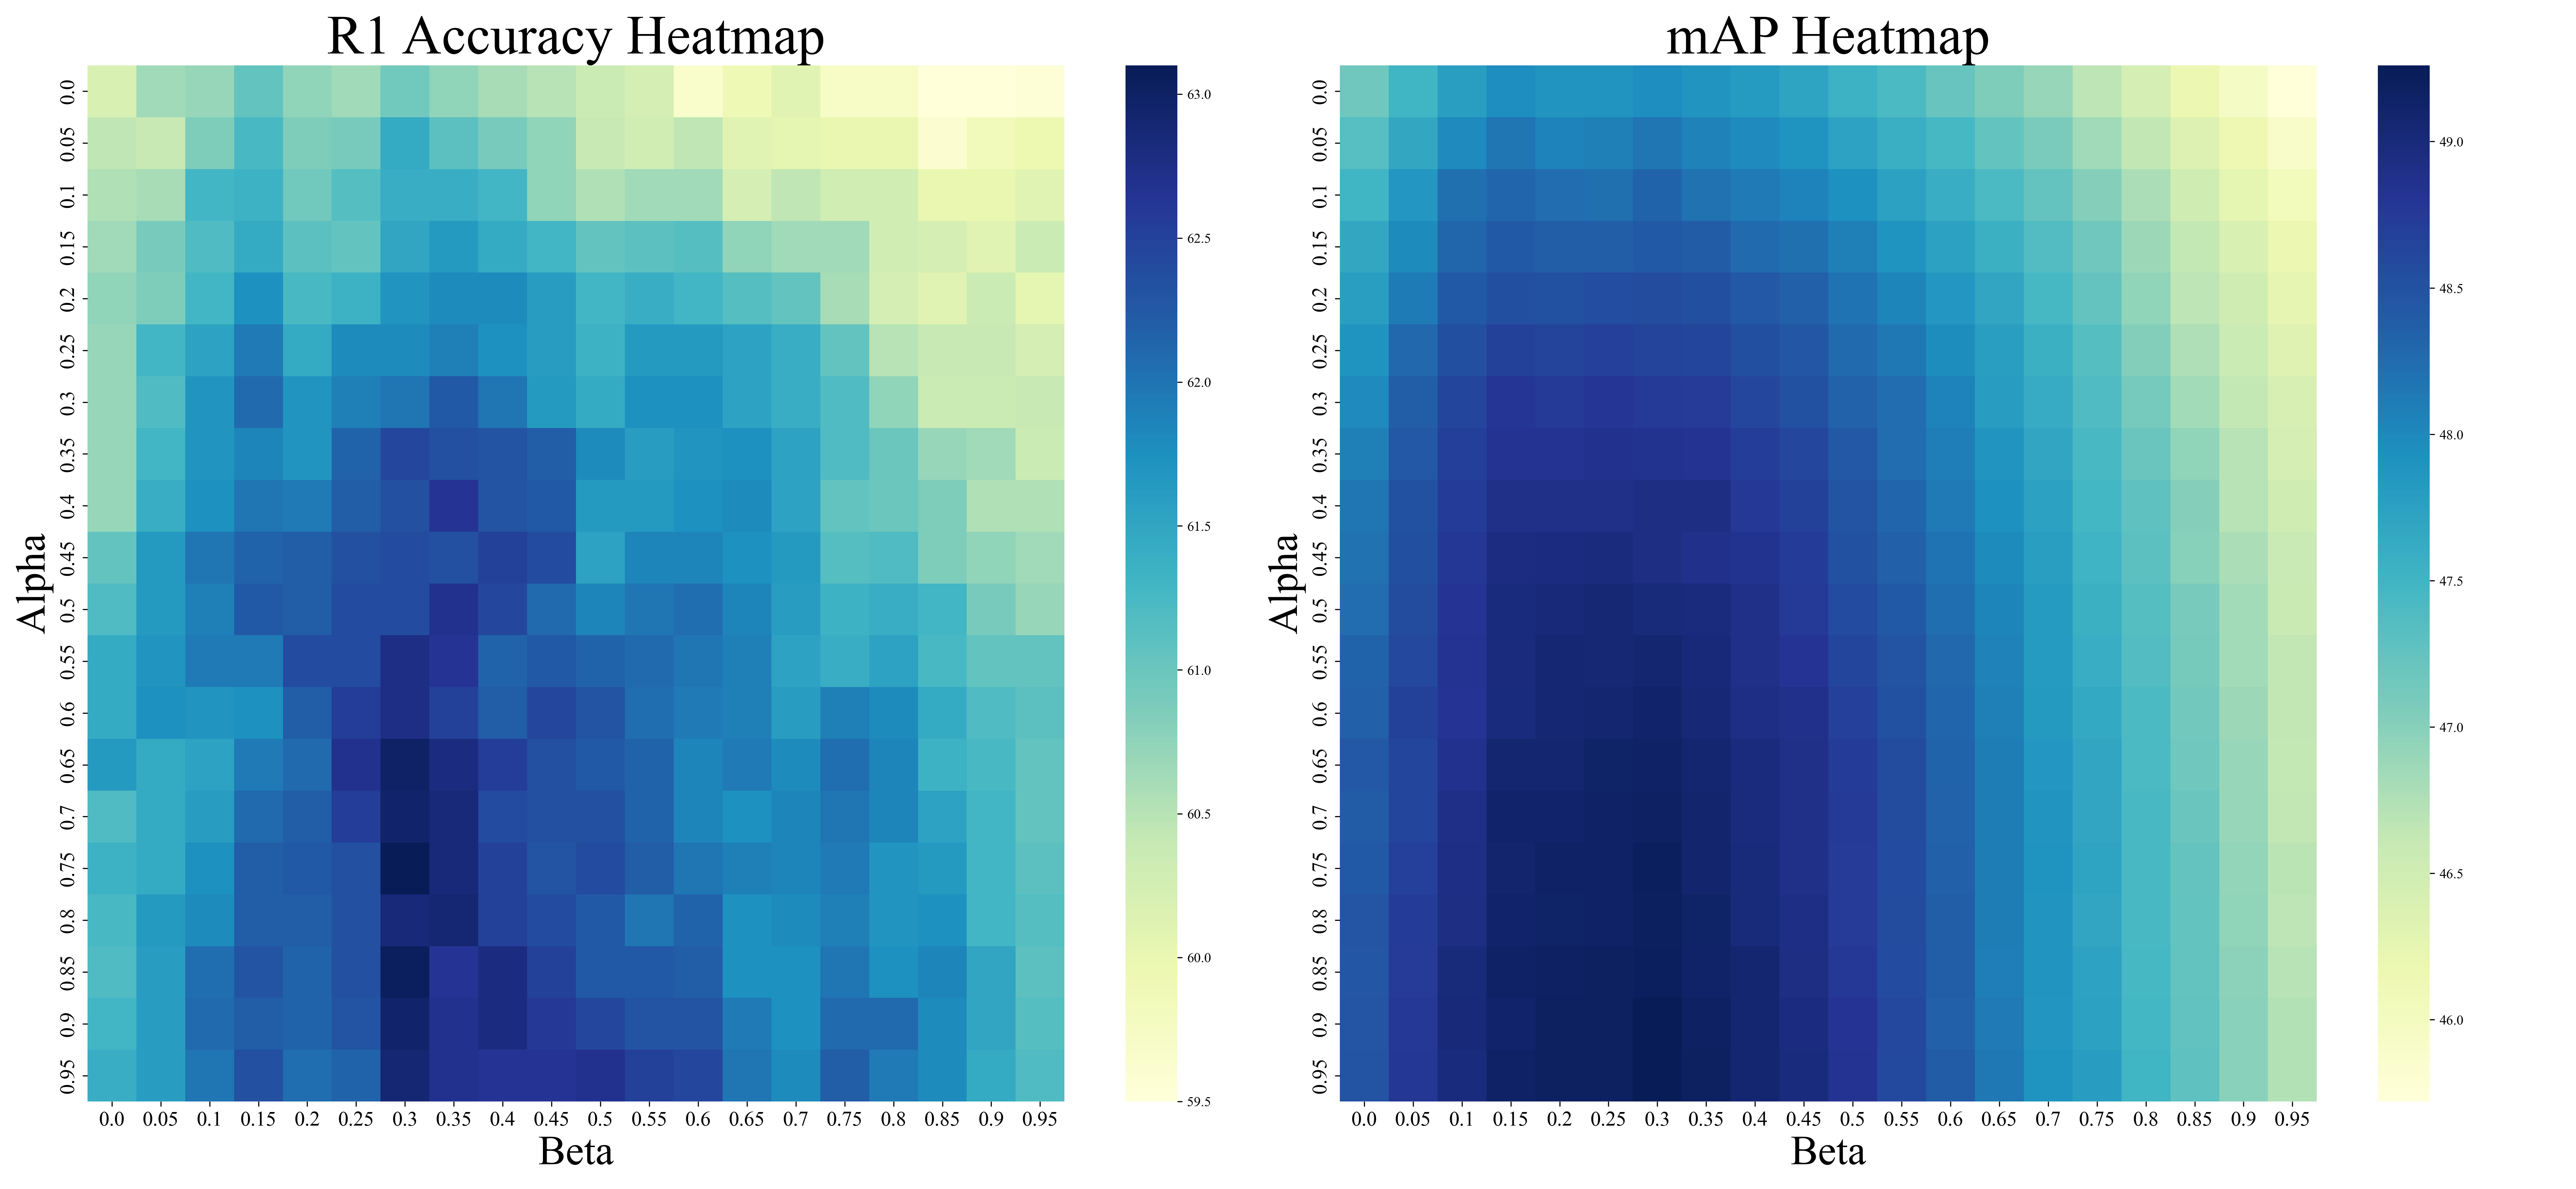
\includegraphics[width=\linewidth]{figs/rank1_map_heatmaps.png}
\caption{Heatmap of R1 accuracy and mAP on the RSTPReid dataset with IRRA baseline.}
\label{fig:heatmap}
\end{figure}

\begin{figure}
\centering
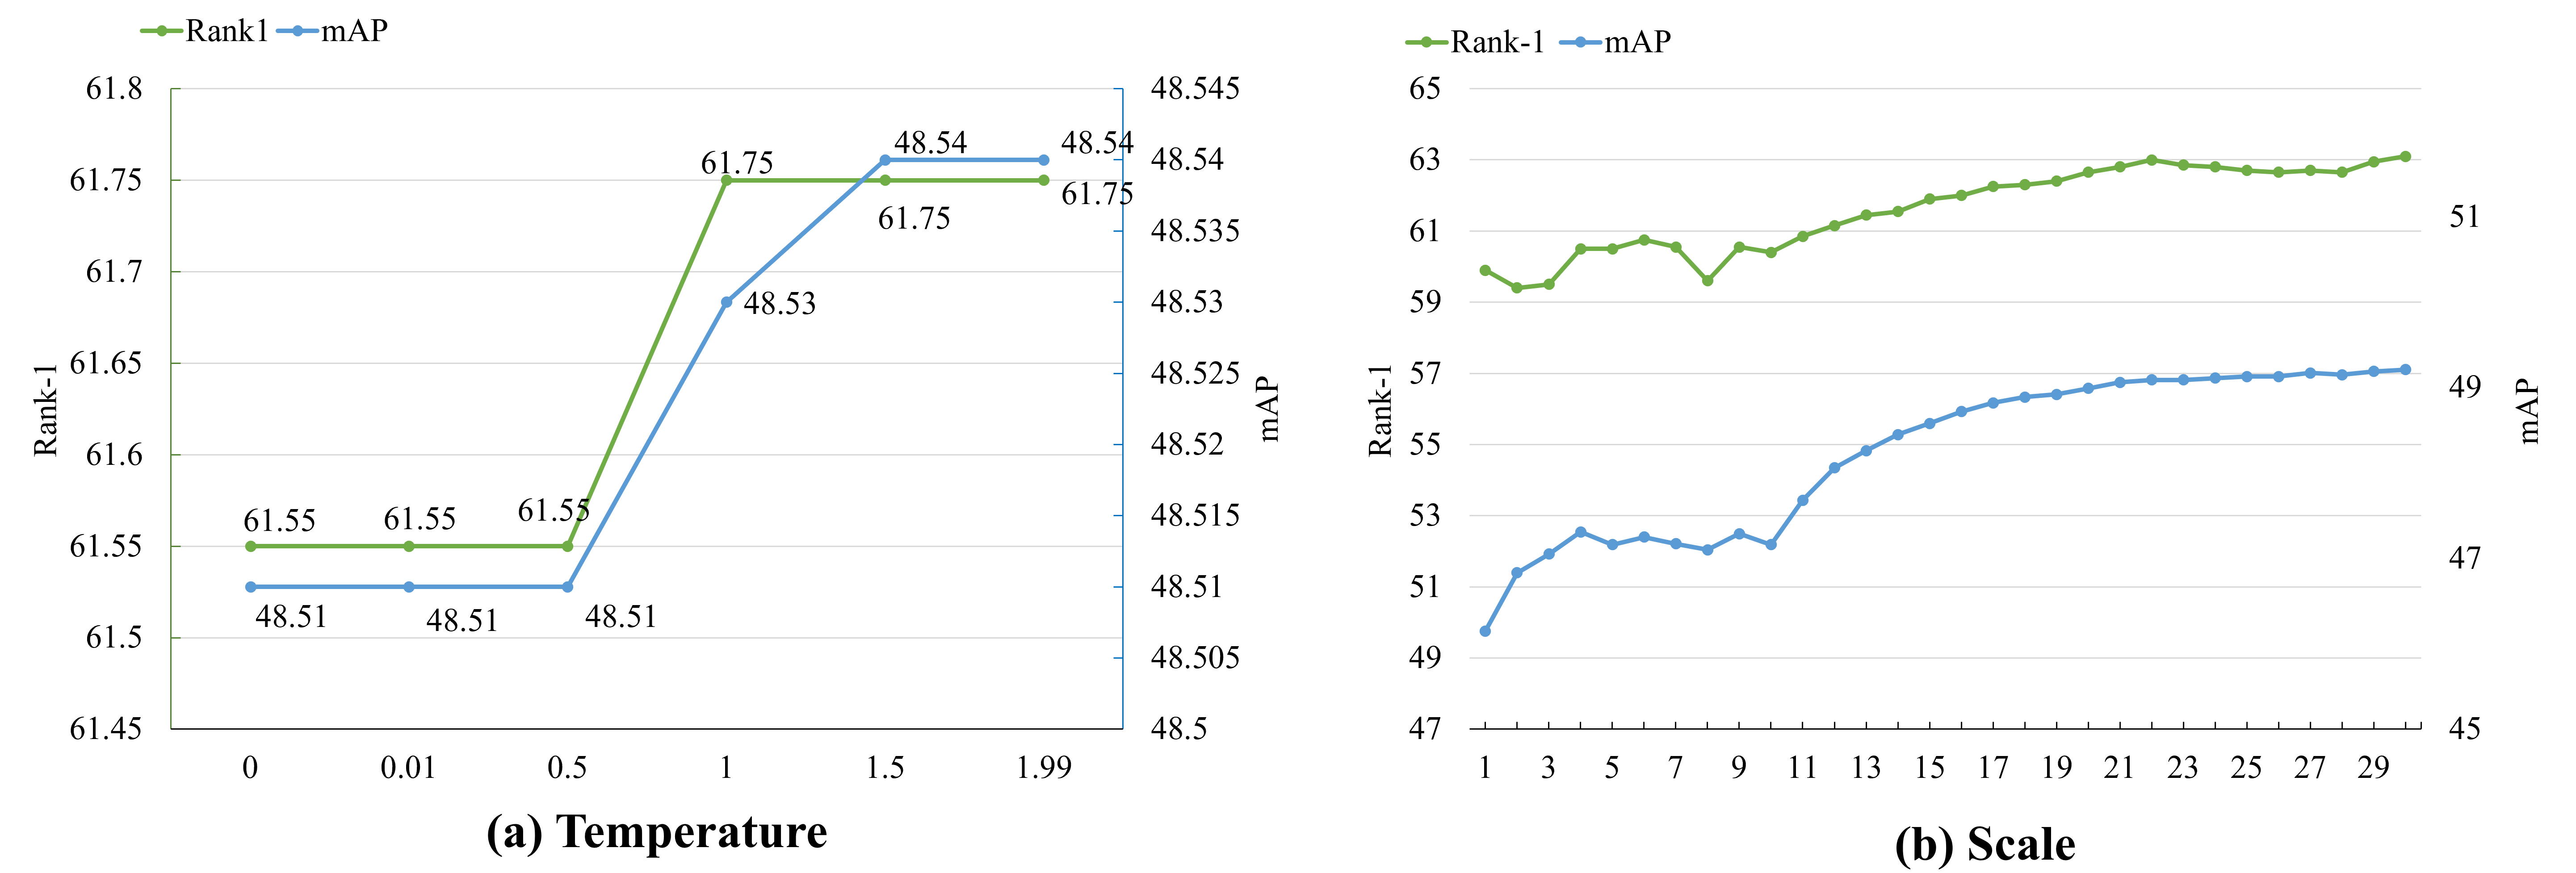
\includegraphics[width=\linewidth]{figs/tem_scale.png}
\caption{(a)Impact of different temperature $\tau$ on RSTPReid dataset with IRRA. (b)Impact of query feature compensation scale on RSTPReid dataset with IRRA baseline.}
\label{fig:tem_scale}
\end{figure}



% \begin{figure}
% \centering
% 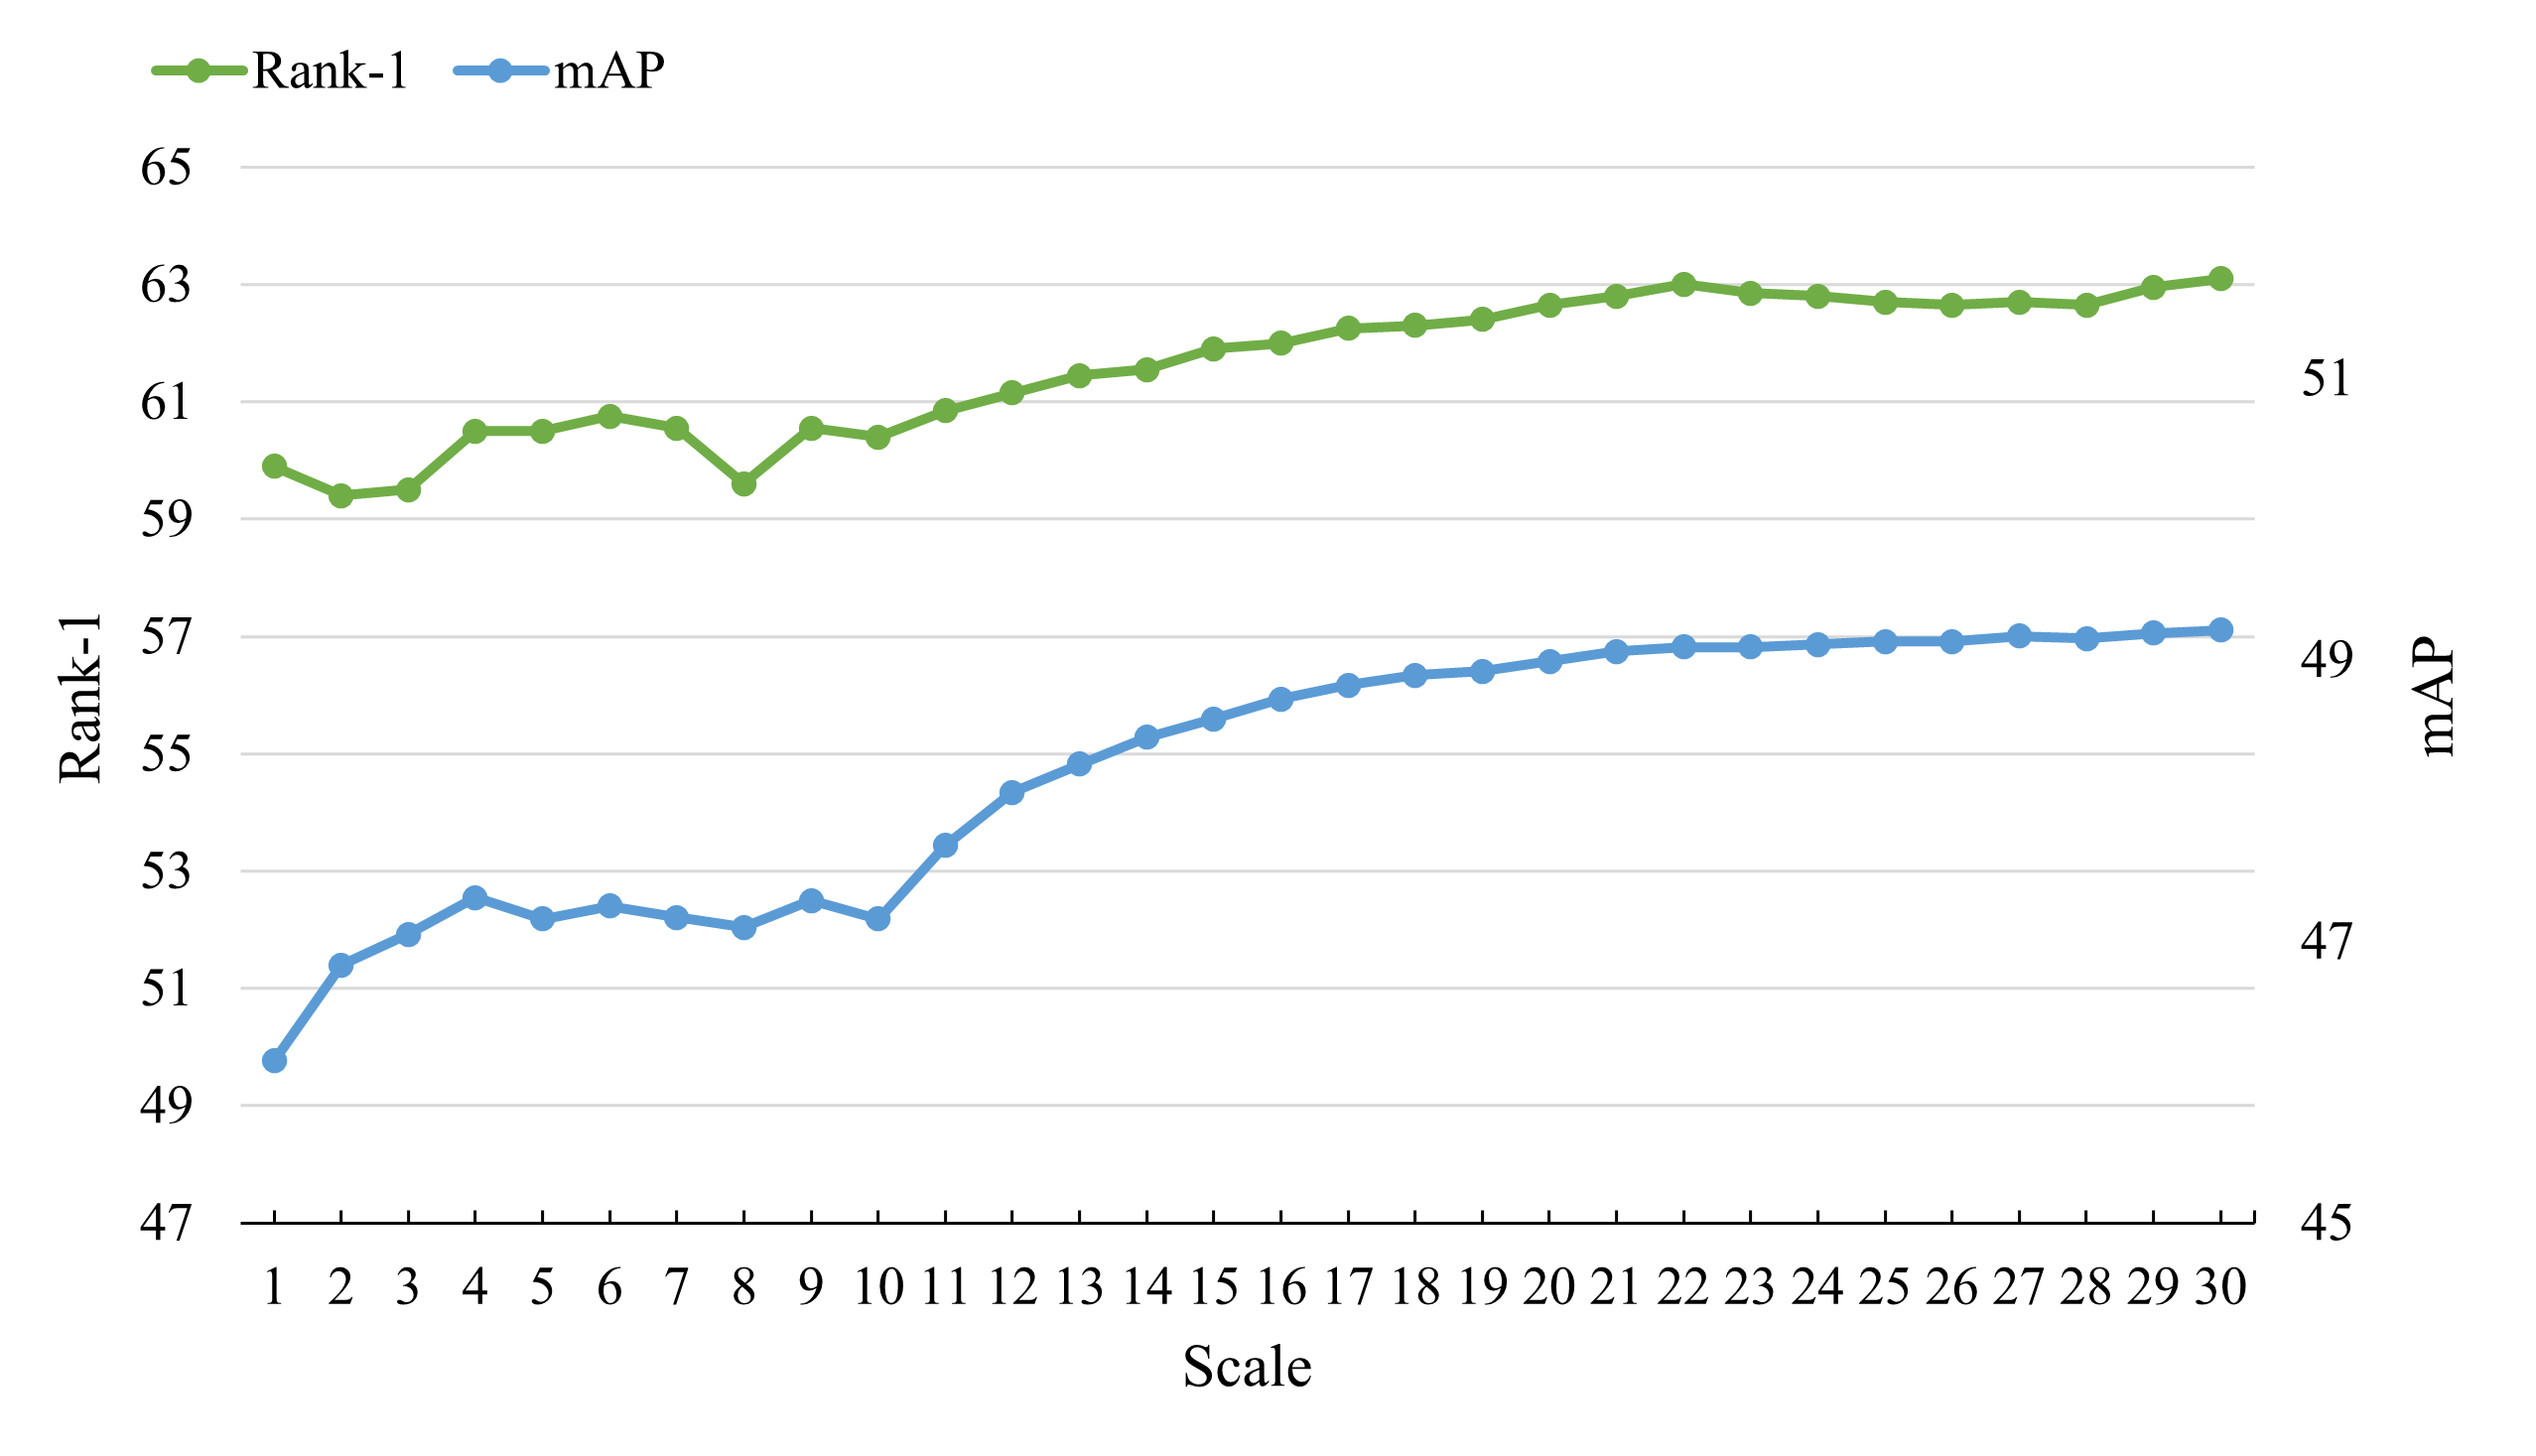
\includegraphics[width=0.95\linewidth]{figs/scale.png}
% \caption{Impact of query feature compensation scale on the RSTPReid dataset with IRRA baseline.}
% \label{fig:scale}
% \end{figure}
\subsection{Comparisons with State-of-the-Art Methods}

We conduct a thorough experimental evaluation comparing our method with recent state-of-the-art approaches across three standard benchmarks: RSTPReid, CUHK-PEDES, and ICFG-PEDES. The comprehensive results, presented in Table ~\ref{tab:sota-traditional}, demonstrate that our method achieves consistent and significant improvements when integrated with various baseline frameworks, establishing new \textbf{state-of-the-art} performance across multiple evaluation metrics.

% Our approach delivers strong results on the RSTPReid dataset. With the IRRA baseline, we achieve a +2.90\% improvement in Rank-1 accuracy, and a +2.25\% boost with the RDE framework. Notably, our method enhances the HAM+RDE framework to 73.75\% Rank-1 accuracy, surpassing the previous best result of 71.65\% from AUL \cite{li2024adaptive} by 2.10\%. These improvements are further reflected in the mAP, underscoring the method's ability to maintain high precision.

% The results on CUHK-PEDES show similar patterns of improvement. Our approach achieves 78.54\% R1 accuracy and 70.22\% mAP, outperforming recent strong competitors. The improvements are consistent across all evaluation metrics, with particularly notable performance at higher ranks, achieving 91.39\% Rank-5 and 95.08\% Rank-10 with HAM(RDE)+ours.

% On the ICFG-PEDES dataset, known for its fine-grained matching challenges, our method demonstrates particularly strong performance. We improve the HAM+RDE baseline from 69.95\% to 70.52\% in Rank-1 accuracy and from 42.72\% to 43.35\% in mAP, while also achieving 84.20\% Rank-5 and 88.67\% Rank-10. These results significantly outperform recent works such as AUL and F-WoRA, highlighting our method's effectiveness in handling detailed textual descriptions and subtle visual differences.

% The consistent improvements across all three datasets and multiple evaluation metrics highlight the robustness and generalizability of our approach. These comprehensive experimental results not only establish new \textbf{state-of-the-art} performance but also validate the effectiveness of our method in addressing key challenges in text-to-image person retrieval, particularly in cross-modal alignment and fine-grained feature matching under real-world conditions.



\subsection{Ablation Study}

To validate the effectiveness of our proposed feature compensation strategy, we conduct a comprehensive ablation study on the RSTPReid dataset using the IRRA baseline, as shown in Table~\ref{tab: ablation}. When no compensation is applied to either the query or gallery features, the baseline achieves 60.20\% R1 accuracy and 47.17\% mAP.

Introducing compensation using keyword-based prompts ($P_{\text{key}}$) leads to performance improvements, achieving 61.80\% R1 and 48.40\% mAP. Likewise, employing diverse prompts ($P_{\text{diversity}}$) yields further gains, with R1 reaching 61.90\% and mAP increasing to 48.58\%.

When compensation with both $P_{\text{key}}$ and $P_{\text{diversity}}$ is applied solely to the query side, performance rises to 61.35\% R1 and 48.43\% mAP, indicating that enhancing the semantic richness of query features is beneficial. Similarly, applying compensation only to the gallery side results in 60.95\% R1 and 47.95\% mAP, demonstrating that gallery-side enrichment also contributes positively.

The most significant improvement is observed when both query and gallery features are jointly compensated using both prompts, achieving 63.10\% R1 and 49.20\% mAP. This represents a relative gain of +2.90\% in R1 and +2.03\% in mAP over the baseline. These results confirm the complementary nature of the two compensation strategies and underscore their effectiveness in addressing the modality gap and semantic misalignment challenges inherent in text-to-image person retrieval.


\begin{table}[tp]
\caption{Comparison of different LLMs for query and gallery feature compensation on RSTPReid with IRRA baseline. The LLMs utilized, in sequential order, are Grok-3, DeepSeek-V3, GPT-4o-Mini, and Qwen2.5-VL-32B.}
\vspace{-0.8em}
\label{tab: different llm}
\centering
\resizebox{0.975\linewidth}{!}{
\begin{tabular}{cccc|cccc}
\hline
\multicolumn{4}{c|}{LLMs}  & \multicolumn{4}{c}{RSTPReid} \\ 

\includegraphics[width=0.03\textwidth]{figs/grok.png} & 
\includegraphics[width=0.03\textwidth]{figs/deepseek.png} & 
\includegraphics[width=0.03\textwidth]{figs/openai.png}& 
\includegraphics[width=0.03\textwidth]{figs/qwen.png}& R1 & R5 & R10 & mAP \\
\hline
\ding{55}& \ding{55}& \ding{55}& \ding{55} & 60.20 & 81.30 & 88.20 & 47.17 \\
 \hline
\ding{52} &\ding{55} &\ding{55} & \ding{55} & 60.95 & 81.15 & 88.55 & 48.08 \\
\ding{55}& \ding{52}& \ding{55}& \ding{55} & 61.10 & 82.00 & 88.95 & 48.19 \\
\ding{55}&\ding{55} & \ding{52}&\ding{55} & 60.95 & 81.85 & 89.20 & 48.18 \\
\ding{55} & \ding{55}& \ding{55}& \ding{52} & 61.55 & 81.75 & 88.9 & 48.51 \\
\hline
\ding{52} & \ding{52} & \ding{55} & \ding{55} & 61.10 & 82.50 & 89.00 & 48.47 \\
\ding{52} & \ding{52} &\ding{52} & \ding{55} & 61.45 & 81.85 & 89.05 & 48.45\\
% \ding{52} & \ding{52} & \ding{55} & \ding{55} & 61.30 & 81.85 & 89.05 & 48.29 \\
% \ding{52} & \ding{52} & \ding{52} & \ding{55} & 61.95 & 81.90 & 88.75 & 48.57 \\
% \ding{52} & \ding{52} & \ding{55} & \ding{52} & 61.30 & 82.00 & 88.95 & 48.54 \\
% \ding{52} & \ding{52} & \ding{55} & \ding{52} & 61.45 & 81.95 & 89.45 & 48.23 \\
\ding{52} & \ding{52} & \ding{52} & \ding{52} & 61.70 & 82.20 & 89.10 & 48.42\\
 \hline
\end{tabular}
}
\end{table}

\begin{figure*}
\centering
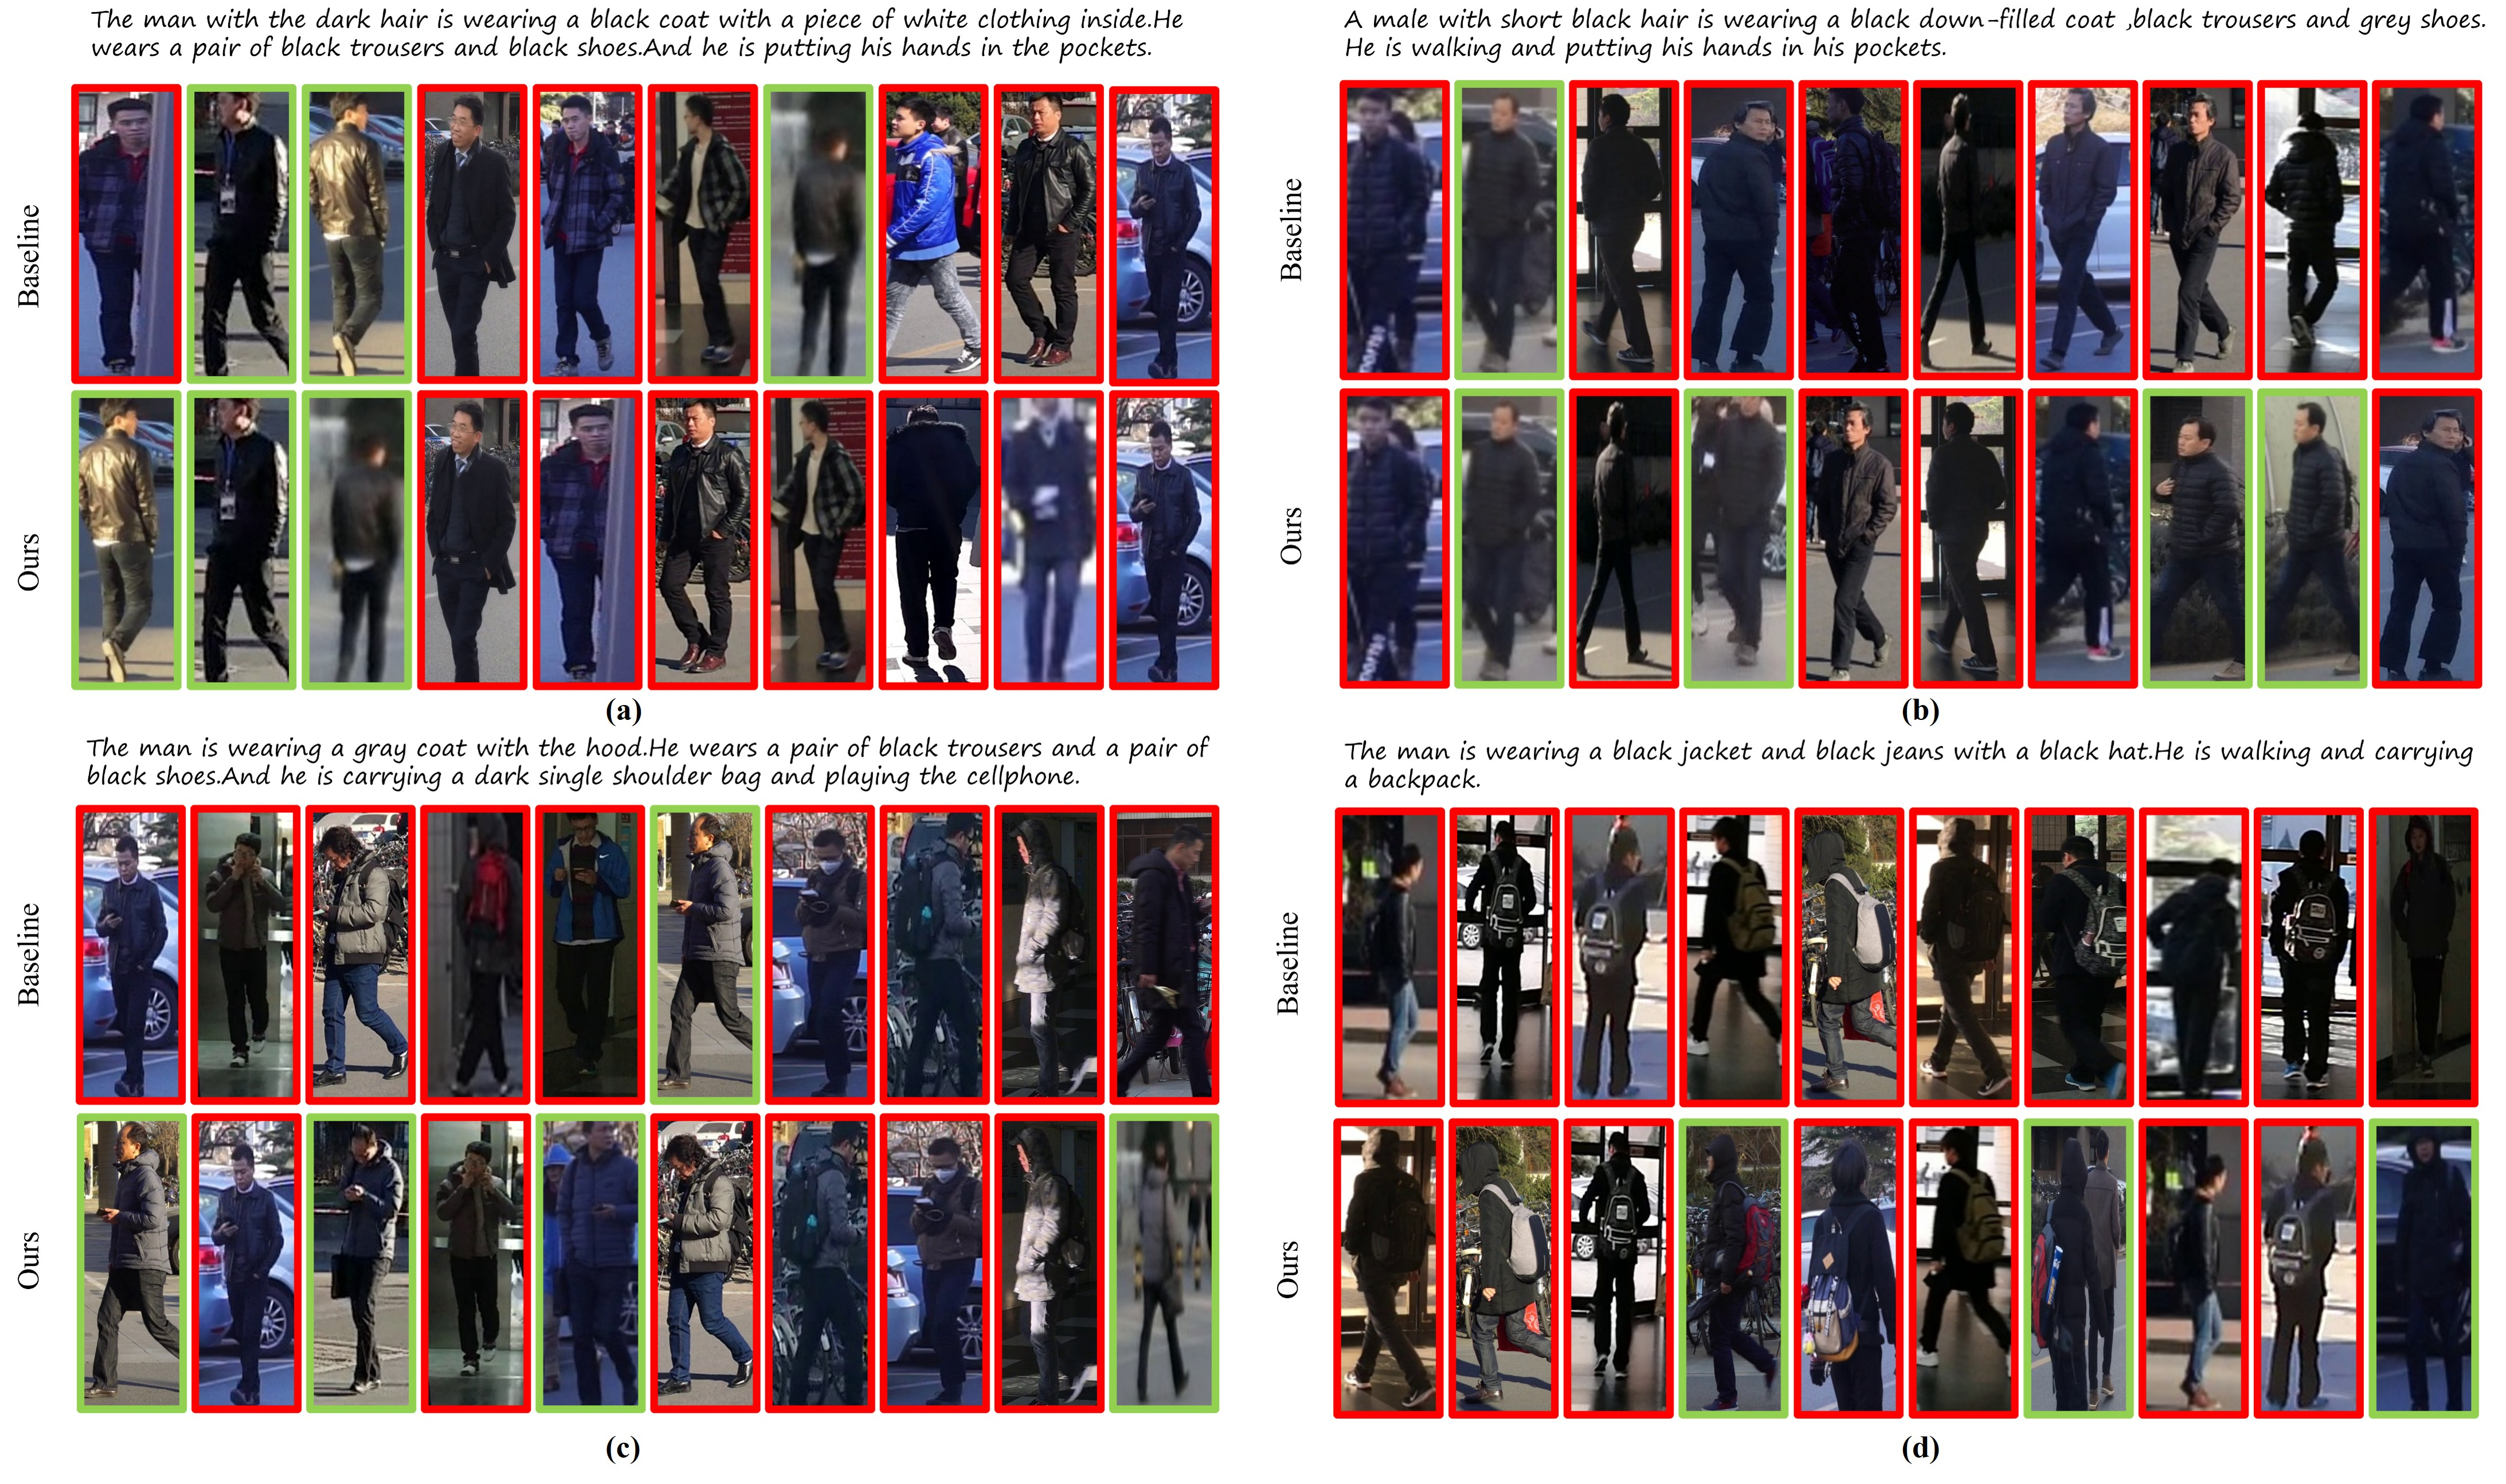
\includegraphics[width=0.9\linewidth]{figs/vis_high_2.jpg}
\caption{Visual comparison of top-10 retrieved results between IRRA(baseline) and our method. Green boxes indicate correct matches, while red boxes are incorrect ones.}
\label{fig:visual}
\end{figure*}

\subsection{Hyperparameter sensitivity analysis}

\textbf{The impact of $\alpha$ and $\beta$.} Our sensitivity analysis in Fig~\ref{fig:heatmap} explores the effect of varying $\alpha$ and $\beta$ on R1 accuracy and mAP. The heatmaps show optimal performance when $\alpha \approx 0.75$ and $\beta \approx 0.3$, where R1 peaks at 63.1\% and mAP at 49.2\%. These results highlight a stable parameter range that maximizes both metrics, demonstrating the robustness of our method. Notably, the dark regions in both heatmaps align, indicating that tuning $\alpha$ and $\beta$ to these values improves retrieval accuracy and precision.

\noindent\textbf{The impact of temperature $\tau$}. To investigate the effect of temperature on caption generation, we vary the temperature of Qwen2.5-VL-32B-Instruct within the range [0,2) and evaluate its performance using the IRRA baseline. As shown in Fig.~\ref{fig:tem_scale}(a), both R1 and mAP remain stable at low temperatures, with R1 at 61.55\% and mAP at 48.51\%. These results suggest that higher temperatures introduce greater diversity in the generated captions, thereby enhancing retrieval performance.

\noindent\textbf{The scalability of our proposed MVR.} To evaluate the scalability of our method, we conducted experiments to examine the impact of varying the query feature compensation scale. The results, shown in Fig.~\ref{fig:tem_scale}(b), illustrate the performance as a function of the scale parameter. As the scale increases, both R1 accuracy and mAP consistently improve, reaching their peak values at the maximum scale of 30. R1 and mAP reach 63.1\% and 49.2\%, respectively. This upward trend demonstrates that our method benefits significantly from larger scales. Such behavior highlights the scalability of our method, as it effectively leverages higher-scale feature compensation to enhance retrieval accuracy. 

% \begin{table}[tp]
% \caption{Comparison of different LLMs for query and gallery feature compensation on RSTPReid with IRRA baseline. The LLMs utilized, in sequential order, are Qwen2.5-VL-32B-Instruct, DeepSeek-V3, GPT-4o-Mini, and Grok-3-Mini-Beta.}
% \vspace{-0.8em}
% \label{tab: different llm}
% \centering
% \resizebox{0.975\linewidth}{!}{
% \begin{tabular}{cccc|cccc}
% \hline
% \multicolumn{4}{c|}{LLM}  & \multicolumn{4}{c}{RSTPReid} \\ 
% 
\includegraphics[width=0.03\textwidth]{figs/qwen.png} & 
\includegraphics[width=0.03\textwidth]{figs/deepseek.png} & 
\includegraphics[width=0.03\textwidth]{figs/openai.png}& 
\includegraphics[width=0.03\textwidth]{figs/grok.png}& R1 & R5 & R10 & mAP \\
% \hline
% \ding{55}& \ding{55}& \ding{55}& \ding{55} & 60.20 & 81.30 & 88.20 & 47.17 \\
%  \hline
% \ding{52} & \ding{55}& \ding{55}& \ding{55} & 61.55 & 81.75 & 88.9 & 48.51 \\
% \ding{55}& \ding{52}& \ding{55}& \ding{55} & 61.10 & 82.00 & 88.95 & 48.19 \\
% \ding{55}&\ding{55} & \ding{52}&\ding{55} & 60.95 & 81.85 & 89.20 & 48.18 \\
% \ding{55} &\ding{55} &\ding{55} & \ding{52} & 60.95 & 81.15 & 88.55 & 48.08 \\
% \hline
% \ding{55} & \ding{52} & \ding{55} & \ding{52} & 61.10 & 82.50 & 89.00 & 48.47 \\
% \ding{55} & \ding{52} &\ding{52} & \ding{52} & 61.45 & 81.85 & 89.05 & 48.45\\
% % \ding{52} & \ding{52} & \ding{55} & \ding{55} & 61.30 & 81.85 & 89.05 & 48.29 \\
% % \ding{52} & \ding{52} & \ding{52} & \ding{55} & 61.95 & 81.90 & 88.75 & 48.57 \\
% % \ding{52} & \ding{52} & \ding{55} & \ding{52} & 61.30 & 82.00 & 88.95 & 48.54 \\
% % \ding{52} & \ding{52} & \ding{55} & \ding{52} & 61.45 & 81.95 & 89.45 & 48.23 \\
% \ding{52} & \ding{52} & \ding{52} & \ding{52} & 61.70 & 82.20 & 89.10 & 48.42\\
%  \hline
% \end{tabular}
% }
% \end{table}




\begin{figure}
\centering

\includegraphics[width=\linewidth]{figs/tsne.png}
\caption{T-sne visualizations of the baseline and ours method. The crosses represent query features and circles represent gallery features.}
\label{fig:tsne}
\end{figure}
\subsection{Effect of different LLMs}

To explore differences in LLM representations, we conducted an interesting experiment demonstrating that leveraging stylistic diversity across different LLMs enhances feature representation, validating our use of diverse rewrites.

Table~\ref{tab: different llm} presents the results of various LLMs for feature compensation on the RSTPReid dataset under the IRRA baseline. Specifically, we assess four representative LLMs: Grok-3\cite{grok3}, DeepSeek-V3 \cite{guo2025deepseek}, GPT-4o-Mini \cite{openai2024gpt4o}, and Qwen2.5-VL-32B \cite{Qwen2.5-VL}, both individually and in combination. Feature compensation is evaluated using the diversity prompt $P_{\text{diversity}}$, with each LLM producing 10 reformulated queries.

% As shown in Table~\ref{tab: different llm}, all four LLMs contribute to consistent improvements over the non-compensated baseline, verifying the effectiveness of diversity-oriented feature compensation. Among the individual models, Qwen2.5-VL-32B achieves the best performance, indicating its strong reasoning ability under the diversity prompt. Moreover, combining multiple LLMs generally leads to further gains. These findings suggest the fusion of different LLMs helps generate more robust and diverse features for text-to-image person retrieval.

As shown in Table~\ref{tab: different llm}, all four LLMs consistently improve over the baseline, confirming the effectiveness of diversity-based feature compensation. Qwen2.5-VL-32B performs best, highlighting its strong reasoning ability. Combining multiple LLMs yields further gains, suggesting enhanced robustness and diversity.




\subsection{Visualization and qualitative analysis.}

\noindent\textbf{The t-sne visualization. } 
Fig.\ref{fig:tsne} shows the distances between query and gallery. The crosses represent query features and circles represent gallery features. It showsthe great capbility of our method to align features between texts and images.

\noindent\textbf{The retrieval visualization. } 
We visualize the comparison of top-10 retrieved results between the IRRA baseline and our proposed MVR method, as illustrated in the Fig ~\ref{fig:visual}. Our method consistently retrieves more correct galleries compared to the baseline. For example, in (b), although the baseline struggles with retrieving visually similar individuals with mismatched clothing, our method accurately localizes the correct identity by leveraging fine-grained attributes such as his pose and clothing characteristics. In (d), our method retrieves three correct matches, whereas the baseline fails to retrieve any. Despite the presence of two pedestrians in the gallery image, our method is still able to accurately extract robust features. These results highlight the advantage of incorporating richer semantic alignment between vision and language features in complex real-world settings.


\subsection{Computational and commercial costs.}

Computational cost includes text generation and feature compensation. Using Qwen2.5-VL-32B, generating test set texts for CUHK-PEDES, ICFG-PEDES, and RSTPReid took 38, 117, and 12 minutes, respectively, on an I9-13900K CPU with 8 threads. Feature compensation on an RTX 4090 GPU is negligible, much lower than training and inference time. Commercial costs refer to API usage fees for the Qwen2.5-VL-32B, totaling \$22, \$61, and \$7 for the CUHK-PEDES, ICFG-PEDES, and RSTPReid datasets, respectively. In summary, the overall computational and commercial costs are minimal.



\section{Conclusion}

In this paper, we propose a training-free LLM-Collaborative Multi-View Reformulation (MVR) framework to enhance the robustness of text-to-image person retrieval under expression drift and visual ambiguity. By leveraging the generative and reasoning capabilities of large language models, we construct multi-view semantic reformulations that are aggregated in latent space to enrich both textual and visual representations. Extensive experiments demonstrate that our method significantly improves retrieval performance. In future work, we plan to extend our framework to multi-modal reasoning tasks beyond retrieval, further leveraging the complementary strengths of language and vision.